\documentclass[aspectratio=169,11pt]{beamer}
\usetheme[progressbar=frametitle,numbering=fraction,sectionpage=none]{metropolis}
\metroset{block=transparent}
\usepackage{amsmath,amssymb,booktabs,tabularx,array,ragged2e,tikz}
\usetikzlibrary{arrows.meta,positioning}
\definecolor{SoftBlue}{RGB}{76,112,150}
\definecolor{BlockBlue}{RGB}{228,236,246}
\definecolor{BlockBlueDark}{RGB}{207,222,239}
\definecolor{SoftGreen}{RGB}{34,110,91}
\definecolor{Accent}{RGB}{169,83,37}
\definecolor{Ink}{RGB}{32,40,52}
\definecolor{Secondary}{RGB}{73,88,104}
\setbeamercolor{normal text}{fg=Ink,bg=white}
\setbeamercolor{structure}{fg=SoftBlue}
\setbeamercolor{frametitle}{fg=Ink,bg=white}
\setbeamercolor{progress bar}{fg=SoftBlue,bg=gray!20}
\setbeamercolor{alerted text}{fg=SoftBlue}
\setbeamercolor{title separator}{fg=SoftBlue}
\setbeamercolor{block title}{fg=Ink,bg=BlockBlueDark}
\setbeamercolor{block body}{fg=Ink,bg=BlockBlue}
\setbeamertemplate{navigation symbols}{}
\AtBeginEnvironment{frame}{\setlength{\parskip}{2pt}\raggedright}
\setbeamersize{text margin left=7mm,text margin right=7mm}
\setbeamerfont{frametitle}{size=\large,series=\bfseries}
\newcolumntype{Y}{>{\RaggedRight\arraybackslash}X}
\newcommand{\kterm}[1]{{\color{SoftBlue}\bfseries #1}}
\newcommand{\lead}[1]{\par{\bfseries\color{SoftBlue}#1}\par}
\newcommand{\notefoot}[1]{\par\vfill{\fontsize{8}{9.3}\selectfont\color{Secondary}#1\par}}
\newcommand{\signal}[1]{\par\smallskip{\color{SoftGreen}\bfseries #1}\par}
\newcommand{\tinyhead}[1]{{\color{Secondary}\footnotesize\bfseries #1}}
\tikzset{edge/.style={-{Stealth},draw=SoftBlue,very thick}, panel/.style={draw=SoftBlue!50,fill=BlockBlue,rounded corners=3pt,align=center,minimum height=.9cm,inner sep=3pt}, norm/.style={draw=SoftBlue,line width=1pt}, fillzone/.style={fill=SoftBlue!23,draw=SoftBlue,line width=.9pt}}
\title{Verified reachability for neural feedback}
\subtitle{How our implementation bounds controller and integration errors}
\date{Project handoff \enspace\textbar\enspace 24 November 2026}
\begin{document}

\begin{frame}[plain]
\vfill
{\color{SoftBlue}\bfseries Project handoff}\par\medskip
{\LARGE\bfseries Verified reachability for neural feedback}\par\medskip
{\large How our implementation bounds controller and integration errors}\par
{\color{SoftBlue}\rule{\linewidth}{.9pt}}\par\smallskip
24 November 2026
\vfill
\end{frame}

\begin{frame}{One control period, from state set to enclosure}
At each controller update, many initial states are possible. The verifier must enclose every trajectory that starts in this set.
\begin{center}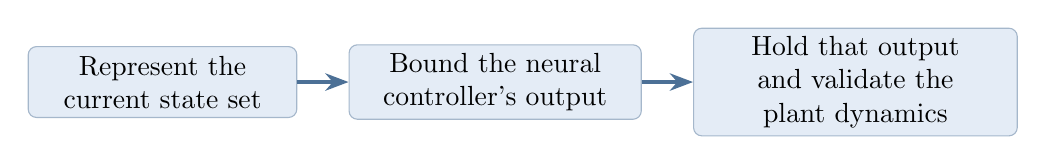
\begin{tikzpicture}
\node[panel,text width=3.2cm](a){Represent the current state set};
\node[panel,text width=3.5cm,right=.65cm of a](b){Bound the neural controller's output};
\node[panel,text width=3.9cm,right=.65cm of b](c){Hold that output and validate the plant dynamics};
\draw[edge](a)--(b);\draw[edge](b)--(c);
\end{tikzpicture}\end{center}
\small
A Taylor model writes a possible state as \(x=P(r)+e\). The vector \(r\) selects an initial condition, the polynomial \(P\) tracks its influence, and the interval containing \(e\) covers the remaining uncertainty.
\signal{The accepted tube covers the entire step. Its endpoint seeds the next step.}
\notefoot{Huan's benchmark implementation uses this same overall procedure. A safety verdict also requires checking the specified property of the reachable states.}
\end{frame}

\begin{frame}{Where our implementation changes the calculation}
\small
\renewcommand{\arraystretch}{1.14}
\noindent\begin{tabularx}{\dimexpr\linewidth-1pt\relax}{@{}p{2.5cm}YY@{}}\toprule
 & \textbf{Huan's benchmark implementation} & \textbf{Our changes in the corresponding stage}\\\midrule
\kterm{Controller} & Inject the affine bound for the whole input box. & Account for rounded coefficients. Optionally tighten the residual at a fixed slope or around a fixed polynomial.\\
\kterm{Integration} & Check a local error box with the same size throughout the step. & Optionally validate an error allowance that grows from the beginning of the step.\\
\kterm{History} & Carry previous remainder increments through point matrix products. & Enclose transport factors and products using interval arithmetic.\\\bottomrule
\end{tabularx}
\notefoot{The comparison refers to the implementation used in the retained experiments. Huan's manuscript also describes strict rounding compensation and other controller bounds.}
\end{frame}

\begin{frame}{Accounting for the coefficients we store}
\small
Huan's injection carries the incoming state error and the gap in the controller bound into the control remainder. Our strict injection also bounds the error in forming the stored polynomial.
\[
\underbrace{J}_{\text{control remainder}}=
\underbrace{TI}_{\text{incoming error}}+
\underbrace{([L,U]-c)}_{\text{controller gap}}+
\underbrace{E_{\rm coeff}}_{\text{coefficient error}}.
\]
The matrix \(T\) is the slope of the affine bound, \(I\) encloses the state error, \([L,U]\) encloses the controller bias, and \(c\) is the bias used in the stored polynomial.
\begin{block}{Suppose coefficients are stored to two decimal places}
A product \(0.25\times0.27=0.0675\) is stored as \(0.07\). Its term multiplies \(r\in[-1,1]\), so the error in the value ranges from \(-0.0025\) to \(0.0025\).
\end{block}
\notefoot{Our code encloses the coefficient operations and evaluates their discrepancy over the parameter domain. This extra calculation makes the rounding contribution explicit.}
\end{frame}

\begin{frame}{Refining the controller residual at a fixed slope}
\small
For controller output \(N(x)\) and a fixed slope \(T\), the residual is \(g(x)=N(x)-Tx\). Huan uses the bound for the whole box. We can subdivide the box and bound the same residual independently on each piece.
\begin{columns}[T,onlytextwidth]
\begin{column}{.48\textwidth}
\lead{Two pieces of the input}
Take \(N(x)=\max(0,x)\), \(T=1\), and \(-1\leq x\leq 1\).
\[
g(x)=\begin{cases}-x& -1\leq x<0,\\0&0\leq x\leq 1.\end{cases}
\]
The left piece yields \([0,1]\), the right yields \(\{0\}\). Their hull is \([0,1]\).
\end{column}
\begin{column}{.48\textwidth}
\lead{Two bounds on the same piece}
Intersect a forward evaluation with a second evaluation that keeps shared activation errors together longer. An error with downstream coefficients \(+3\) and \(-3\) cancels when combined first.
\end{column}
\end{columns}
\notefoot{The extra subbox evaluations can tighten the residual. The retained plugin supports four inputs, two hidden layers of 25 rectified neurons each, and two outputs.}
\end{frame}

\begin{frame}{An independent bound around the same control polynomial}
\small
After injection, Huan uses the resulting control remainder. Our anchor step obtains another affine certificate and measures both bounds relative to the \emph{same stored polynomial} \(V\).
\[
\underbrace{N(x)-V(x)}_{\text{same discrepancy}}\ \in\ 
\underbrace{J_{\rm original}\cap J_{\rm independent}}_{\text{remainder carried forward}}.
\]
\begin{block}{Use the same controller as on the previous slide}
Let \(N(x)=\max(0,x)\), \(V(x)=x/2\), and \(-1\le x\le1\). Their difference equals \(|x|/2\). Intersecting an original bound \([-0.5,1]\) with the independent bound \([0,0.5]\) leaves \([0,0.5]\).
\end{block}
\signal{Fixed-slope refinement can move the constant term. Anchoring keeps every stored coefficient fixed.}
\notefoot{The selected Quadrotor run made 50 original and 50 independent controller-bound calls.}
\end{frame}

\begin{frame}{Validating an error tube that grows with time}
\small
Huan tests an error box of constant size on the local step. Our optional check starts a fresh polynomial at the incoming set and proposes an allowance proportional to elapsed time.
\begin{columns}[T,onlytextwidth]
\begin{column}{.47\textwidth}\centering\tinyhead{Constant allowance}\par
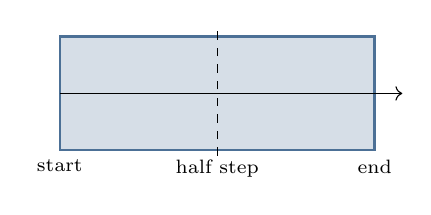
\begin{tikzpicture}[x=1cm,y=.72cm]\filldraw[fillzone](0,-1)rectangle(4,1);\draw[->](0,0)--(4.35,0);\draw[dashed](2,-1.1)--(2,1.15);\node[below,font=\scriptsize] at(0,-1){start};\node[below,font=\scriptsize] at(2,-1){half step};\node[below,font=\scriptsize] at(4,-1){end};\end{tikzpicture}
\end{column}
\begin{column}{.49\textwidth}\centering\tinyhead{Time-weighted allowance}\par
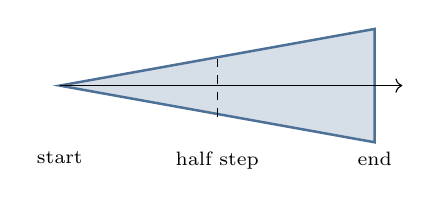
\begin{tikzpicture}[x=1cm,y=.72cm]\filldraw[fillzone](0,0)--(4,1)--(4,-1)--cycle;\draw[->](0,0)--(4.35,0);\draw[dashed](2,-.55)--(2,.55);\node[below,font=\scriptsize] at(0,-1){start};\node[below,font=\scriptsize] at(2,-1){half step};\node[below,font=\scriptsize] at(4,-1){end};\end{tikzpicture}
\end{column}
\end{columns}
At half a step, an endpoint allowance of \(\pm0.02\) becomes \(\pm0.01\). Acceptance requires proving that the computed integration defect fits the proposed tube.
\notefoot{The initial local discrepancy is zero only when the new polynomial matches its seed. The seed retains the full incoming uncertainty. Each weighted check adds a field evaluation.}
\end{frame}

\begin{frame}{Transporting earlier errors with interval factors}
\small
Both implementations keep earlier remainder increments. A transport matrix describes how an old increment affects the current state. Huan stores point products. Our strict history carries interval factors and multiplies them outward.
\begin{block}{One old error in \([0,3]\), with an exact factor of one third}
\renewcommand{\arraystretch}{1.18}
\noindent\begin{tabularx}{\dimexpr\linewidth-8pt\relax}{@{}Yr@{}}
Exact product & \((1/3)[0,3]=[0,1]\)\\
Stored point approximation, before any compensation & \(0.33[0,3]=[0,0.99]\)\\
Two-decimal interval factor & \([0.33,0.34][0,3]=[0,1.02]\)
\end{tabularx}
\end{block}
The interval product includes the exact upper endpoint. A point implementation can carry its rounding contribution separately. Huan's manuscript describes such compensation.
\notefoot{In the strict history implementation each factor uses endpoint polynomial linear coefficients and inverse normalization scales. Interval matrix products cost work and can widen the enclosure.}
\end{frame}

\begin{frame}{What the Double Pendulum ablations establish}
\small
Three independent runs changed one mechanism at a time on the less-robust controller. Each used the same degree settings \((4,3,3)\) and retained required validation.
\par\smallskip
\renewcommand{\arraystretch}{1.29}
\noindent\begin{tabularx}{\dimexpr\linewidth-1pt\relax}{@{}Yrc@{}}\toprule
\textbf{Single change to our configuration} & \textbf{Completed steps} & \textbf{Observed result}\\\midrule
Use the whole-box affine controller bound & 58 of 100 & Next step refused\\
Re-anchor history after every completed step & 29 of 100 & Next step refused\\
Omit optional early weighted tightening & 100 of 100 & All eight width targets met\\\bottomrule
\end{tabularx}\par\smallskip
In this experiment, the first two replacements lost full-horizon completion. The third retained it using ordinary validation with zero weighted maps.
\notefoot{Each row is one scientific run. The eight targets are endpoint and maximum tube width for each of four states. Only a complete run supplies all eight full-horizon widths.}
\end{frame}

\begin{frame}{Why Huan is fast and what transferred}
\begin{columns}[T,onlytextwidth]
\begin{column}{.47\linewidth}
\lead{Execution shared with Huan}
Sparse polynomial supports store active monomials. Specialized plans schedule their operations. Native executors and reusable buffers reduce repeated setup and memory allocation.
\smallskip\par
Huan and Xiangru share core numerical routines. Their batching and orchestration differ.
\end{column}
\begin{column}{.49\linewidth}
\lead{Extra work on our transferred path}
For the less-robust Double Pendulum, one controller update covers 225 boxes with 256 subdivisions each. Over 20 updates the residual evaluator processes \textbf{1,152,000} subboxes.
\smallskip\par
The original network verifier is called \textbf{20 times}. The additional work happens inside the residual evaluator.
\end{column}
\end{columns}
\notefoot{Operation counts describe work performed. The retained timings measure the entire configuration. No exclusive timing breakdown assigns a duration to every mechanism.}
\end{frame}

\begin{frame}{What changes when the degrees are matched}
\small
Read \((w,p,v)\) as the degrees for \kterm{working polynomial storage}, \kterm{point expansion} to build a candidate, and \kterm{validation expansion} to check it. Our earlier \((3,2,4)\) was an implementation setting.
\par\smallskip
\renewcommand{\arraystretch}{1.25}
\noindent\begin{tabularx}{\dimexpr\linewidth-1pt\relax}{@{}p{2.95cm}Y Y@{}}\toprule
 & \textbf{At Huan's saved degrees} & \textbf{Our selected degrees}\\\midrule
Double Pendulum, less robust & \((4,3,3)\) permits a complete no-early-weighted run. & \((3,2,3)\) completes 100 steps with zero weighted maps.\\
Quadrotor & \((2,1,1)\) accepts 600 steps. Step 601 is refused. & \((3,2,2)\) accepts all 1,000 steps.\\\bottomrule
\end{tabularx}
\notefoot{Degree matching controls three common inputs. Module settings, arithmetic and execution costs can still differ. The selected configurations come from a bounded search over legal settings.}
\end{frame}

\begin{frame}{Recorded running time}
\small
Three completed cases illustrate a speed gain, a width--time tradeoff, and a costlier recovery of full-horizon completion. Entries are seconds.
\par\smallskip
\renewcommand{\arraystretch}{1.32}
\noindent\begin{tabularx}{\dimexpr\linewidth-1pt\relax}{@{}Yrrrr@{}}\toprule
 & \textbf{Our method} & \textbf{Huan} & \textbf{Xiangru} & \textbf{Flow*}\\\midrule
Unicycle & \kterm{4.30} & 4.80 & 4.80 & 7.52$^\dagger$\\
Double Pendulum, less robust & 4.79 & 3.51 & 3.49 & 821.81\\
Quadrotor & 130.57 & 63.43 & 68.29 & 4,061.10$^\dagger$\\\bottomrule
\end{tabularx}\par\smallskip
Our times are medians of three driver measurements. Huan's Double Pendulum time is also a three-run median. Other Huan and Xiangru entries are individual driver measurements.
\notefoot{Flow* entries are single historical process measurements with capture. $^\dagger$The historical Unicycle and Quadrotor solve different equations or disturbance models and are excluded from direct rankings.}
\end{frame}

\begin{frame}{Where each method gives the narrowest enclosure}
\small
Each pair counts states attaining the smallest \kterm{endpoint width / maximum tube width}. Exact ties credit every tied method.
\par\smallskip
\renewcommand{\arraystretch}{1.19}
\noindent\begin{tabularx}{\dimexpr\linewidth-1pt\relax}{@{}Yrrrr@{}}\toprule
Physical states & \textbf{Our method} & \textbf{Huan} & \textbf{Xiangru} & \textbf{Flow*}\\\midrule
Unicycle (4) & \kterm{4 / 4} & 0 / 0 & 0 / 0 & Different task\\
Double Pendulum, less robust (4) & \kterm{4 / 4} & 0 / 0 & 0 / 0 & 0 / 0\\
Quadrotor (12) & 0 / 1 & 12 / 11 & 12 / 11 & Different task\\\bottomrule
\end{tabularx}\par\smallskip
For the first Unicycle state, the endpoint width was \textbf{0.04294} for our method and \textbf{0.09124} for Huan. Maximum tube widths were \textbf{0.15230} and \textbf{0.18415}, respectively.
\notefoot{Width is upper minus lower after pooling initial boxes at one recorded step. The endpoint uses the final state. For the tube statistic, take the maximum pooled tube width over the saved steps of the complete nominal schedule.}
\end{frame}

\begin{frame}{What remains open across the benchmark suite}
\small
Our selected configurations completed \kterm{20 of 24 numerical schedules}.
\par\smallskip
\renewcommand{\arraystretch}{1.22}
\noindent\begin{tabularx}{\dimexpr\linewidth-1pt\relax}{@{}p{3.27cm}rY@{}}\toprule
\textbf{Case} & \textbf{Completed steps} & \textbf{How to read the record}\\\midrule
Continuous Airplane & 1 of 200 & An exact boundary calculation found a real-model counterexample.\\
Discrete Airplane & 2 of 20 & The retained map configuration covers a short prefix.\\
Cart-pole & 117 of 2,000 & The longest selected prefix ends before the horizon.\\
Double Pendulum, more robust & 72 of 80 & All 225 lanes passed step 72. The property monitor stopped the run.\\\bottomrule
\end{tabularx}
\notefoot{Read each property verdict separately. Some completed cases have no saved state widths.}
\end{frame}

\begin{frame}{How to reproduce a benchmark and check the evidence}
\small
\lead{1. Select one task and configuration}
Use \texttt{docs/handoff/README.md} and \texttt{docs/handoff/results.json} to identify the task, controller, selected configuration and run identifiers.
\smallskip
\lead{2. Trace the numerical route}
Open \texttt{research/handoff\_method/README.md} for the source map. A full rerun needs the matching controller files, device environment and source configuration.
\smallskip
\lead{3. Reconcile a fresh result}
Match accepted steps, property verdict and enabled checks. Compare the same states and horizon. Time the same execution boundary with the same reporting mode.
\notefoot{The local review suite runs on a central processor. The full experiment also uses assets and raw trajectories held on the graphics-processor server.}
\end{frame}

\begin{frame}{What the next maintainer should take from this handoff}
\small
\lead{The gain depends on where uncertainty enters}
The selected Unicycle and less-robust Double Pendulum runs gave the narrowest endpoint and tube widths for all four states in each case.
\smallskip
\lead{The cost depends on which checks actually execute}
The selected Double Pendulum ran zero weighted maps. Quadrotor used independent controller bounds and completed the schedule, with longer runtime and mostly wider enclosures than Huan.
\smallskip
\lead{The first reproduction target}
The less-robust Double Pendulum has a complete trajectory, single-mechanism comparisons and repeated driver timings. Reproduce that configuration before changing a mechanism.
\end{frame}
\end{document}
